\documentclass{beamer}

\usepackage[utf8]{inputenc}
\usepackage{graphicx}
\graphicspath{ {./Figures/} }

\title{Modeling Price and Popularity of AirBnB listings in New-York}
\author{Melody Jiang, Raphael Morsomme, Ezinne Nwankwo}
\institute{Department of Statistical Science, Duke University}
\date{02/03/2020}

\begin{document}

\frame{\titlepage}




\begin{frame}
\frametitle{Results - Random Forest Price}
% latex table generated in R 3.6.1 by xtable 1.8-4 package
% Mon Feb  3 21:05:30 2020
\begin{table}[ht]
\centering
\begin{tabular}{rlr}
  \hline
 & Predictors & Variable.Importance \\ 
  \hline
1 & last\_review & 978.10 \\ 
  2 & name\_listing\_sentiment & 107.88 \\ 
  3 & name\_host\_freq & 101.15 \\ 
  4 & availability\_365 & 100.73 \\ 
  5 & Room\_type & 95.16 \\ 
  6 & number of reviews & 94.24 \\ 
  7 & reviews\_per\_month & 90.71 \\ 
  8 & proximity\_metro & 89.26 \\ 
  9 & calculated\_host\_listings\_count & 88.53 \\ 
  10 & Neighbourhood\_group & 61.00 \\ 
  11 & type\_stay & 53.69 \\ 
  12 & name\_host\_special & 47.78 \\ 
  13 & name\_listing\_length & 39.16 \\ 
  14 & proximity\_attraction & 16.42 \\ 
   \hline
\end{tabular}
\end{table}

\end{frame}

\begin{frame}
\frametitle{Results - Random Forest Popularity}
% latex table generated in R 3.6.1 by xtable 1.8-4 package
% Mon Feb  3 21:49:38 2020
\begin{table}[ht]
\centering
\begin{tabular}{rlr}
  \hline
 & Predictors & Variable.Importance \\ 
  \hline
1 & number\_of\_reviews & 199.74 \\ 
  2 & latitude & 62.77 \\ 
  3 & listing\_sentiment & 59.50 \\ 
  4 & minimum\_nights & 57.85 \\ 
  5 & neighbourhood\_group & 54.93 \\ 
  6 & room\_type & 50.03 \\ 
  7 & reviews\_per\_month & 49.69 \\ 
  8 & longitude & 45.87 \\ 
  9 & name\_listing\_length & 41.50 \\ 
  10 & name\_host\_special & 35.34 \\ 
  11 & popularity\_log & 33.77 \\ 
  12 & proximity\_attraction & 20.73 \\ 
  13 & listing\_count & 8.76 \\ 
  14 & name\_host\_freq & 8.72 \\ 
  15 & proximity\_metro & 0.42 \\ 
   \hline
\end{tabular}
\end{table}

\end{frame}

\begin{frame}
\frametitle{Results - BMA Price}
% latex table generated in R 3.6.1 by xtable 1.8-4 package
% Mon Feb  3 21:53:08 2020
\begin{table}[ht]
\centering
\begin{tabular}{rlrrrl}
  \hline
 & Predictors & Estimate & Lower.Confint & Upper.Confint & Signifance \\ 
  \hline
1 & Intercept & 4.70 & 4.70 & 4.71 & * \\ 
  2 & Neighbourhood\_group:Manhattan & 0.17 & 0.15 & 0.18 & * \\ 
  3 & Neighbourhood\_group:Queens & -0.11 & -0.13 & -0.10 & * \\ 
  4 & Neighbourhood\_group:Staten Island & -0.00 & 0.00 & 0.00 &  \\ 
  5 & Neighbourhood\_group:Bronx & -0.17 & -0.20 & -0.14 & * \\ 
  6 & Room\_type:Entire home/apt & 0.74 & 0.73 & 0.75 & * \\ 
  7 & Room\_type:Shared room & -0.51 & -0.54 & -0.47 & * \\ 
  8 & number of reviews & -0.01 & -0.02 & -0.01 & * \\ 
  9 & last\_review & -0.00 & -0.00 & -0.00 & * \\ 
  10 & reviews\_per\_month & -0.00 & -0.00 & 0.00 &  \\ 
  11 & calculated\_host\_listings\_count & -0.01 & -0.02 & -0.01 & * \\ 
  12 & availability\_365 & 0.00 & 0.00 & 0.00 & * \\ 
  13 & name\_listing\_sentiment & 0.00 & 0.00 & 0.00 & * \\ 
  14 & proximity\_attraction & -0.01 & -0.04 & 0.00 &  \\ 
  15 & name\_host\_freq & 0.07 & 0.07 & 0.07 & * \\ 
  16 & name\_host\_special:True & 10.42 & 7.29 & 13.45 & * \\ 
  17 & name\_listing\_length & 0.06 & 0.04 & 0.08 & * \\ 
  18 & type\_stay:Long & 0.00 & 0.00 & 0.00 & * \\ 
  19 & proximity\_metro & -0.00 & -0.00 & 0.00 &  \\ 
   \hline
\end{tabular}
\end{table}

\end{frame}

\begin{frame}
\frametitle{Results - BMA Popularity}
% latex table generated in R 3.6.1 by xtable 1.8-4 package
% Mon Feb  3 21:53:10 2020
\begin{table}[ht]
\centering
\begin{tabular}{rlrrrl}
  \hline
 & Predictors & Estimate & Lower.Confint & Upper.Confint & Signifance \\ 
  \hline
1 & Intercept & 4.70 & 4.70 & 4.71 & * \\ 
  2 & Neighbourhood\_group:Manhattan & 0.17 & 0.15 & 0.18 & * \\ 
  3 & Neighbourhood\_group:Queens & -0.11 & -0.13 & -0.10 & * \\ 
  4 & Neighbourhood\_group:Staten Island & -0.00 & 0.00 & 0.00 &  \\ 
  5 & Neighbourhood\_group:Bronx & -0.17 & -0.20 & -0.14 & * \\ 
  6 & Room\_type:Entire home/apt & 0.74 & 0.73 & 0.75 & * \\ 
  7 & Room\_type:Shared room & -0.51 & -0.54 & -0.47 & * \\ 
  8 & number of reviews & -0.01 & -0.02 & -0.01 & * \\ 
  9 & last\_review & -0.00 & -0.00 & -0.00 & * \\ 
  10 & reviews\_per\_month & -0.00 & -0.00 & 0.00 &  \\ 
  11 & calculated\_host\_listings\_count & -0.01 & -0.02 & -0.01 & * \\ 
  12 & availability\_365 & 0.00 & 0.00 & 0.00 & * \\ 
  13 & name\_listing\_sentiment & 0.00 & 0.00 & 0.00 & * \\ 
  14 & proximity\_attraction & -0.01 & -0.04 & 0.00 &  \\ 
  15 & name\_host\_freq & 0.07 & 0.07 & 0.07 & * \\ 
  16 & name\_host\_special:True & 10.42 & 7.29 & 13.45 & * \\ 
  17 & name\_listing\_length & 0.06 & 0.04 & 0.08 & * \\ 
  18 & type\_stay:Long & 0.00 & 0.00 & 0.00 & * \\ 
  19 & proximity\_metro & -0.00 & -0.00 & 0.00 &  \\ 
   \hline
\end{tabular}
\end{table}

\end{frame}


\begin{frame}
\frametitle{Diagnostic Plots - BMA}
\includegraphics[scale = 0.8]{diagnostic_price_bma.jpeg}
\includegraphics[scale = 0.8]{diagnostic_pop_bma.jpeg}
\begin{itemize}
	\item Used $R^2$ to diagnose random forest models
\end{itemize}
\end{frame} 

\begin{frame}
\frametitle{Residuals - BMA}
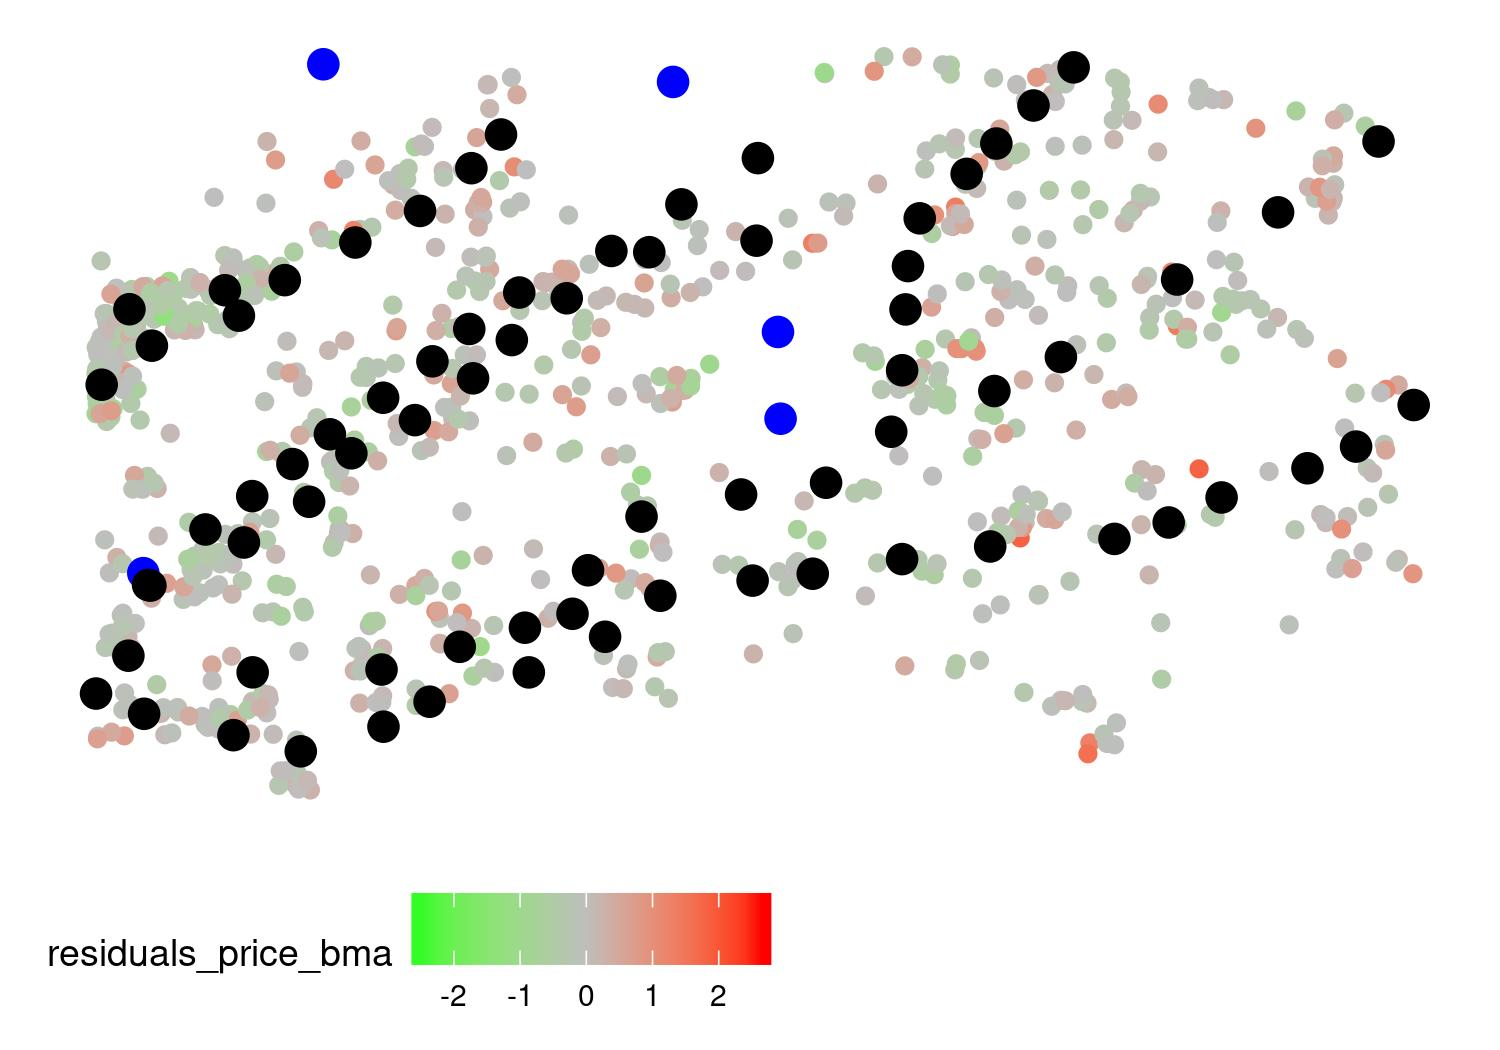
\includegraphics[scale = 0.8]{map_price_bma.jpeg}
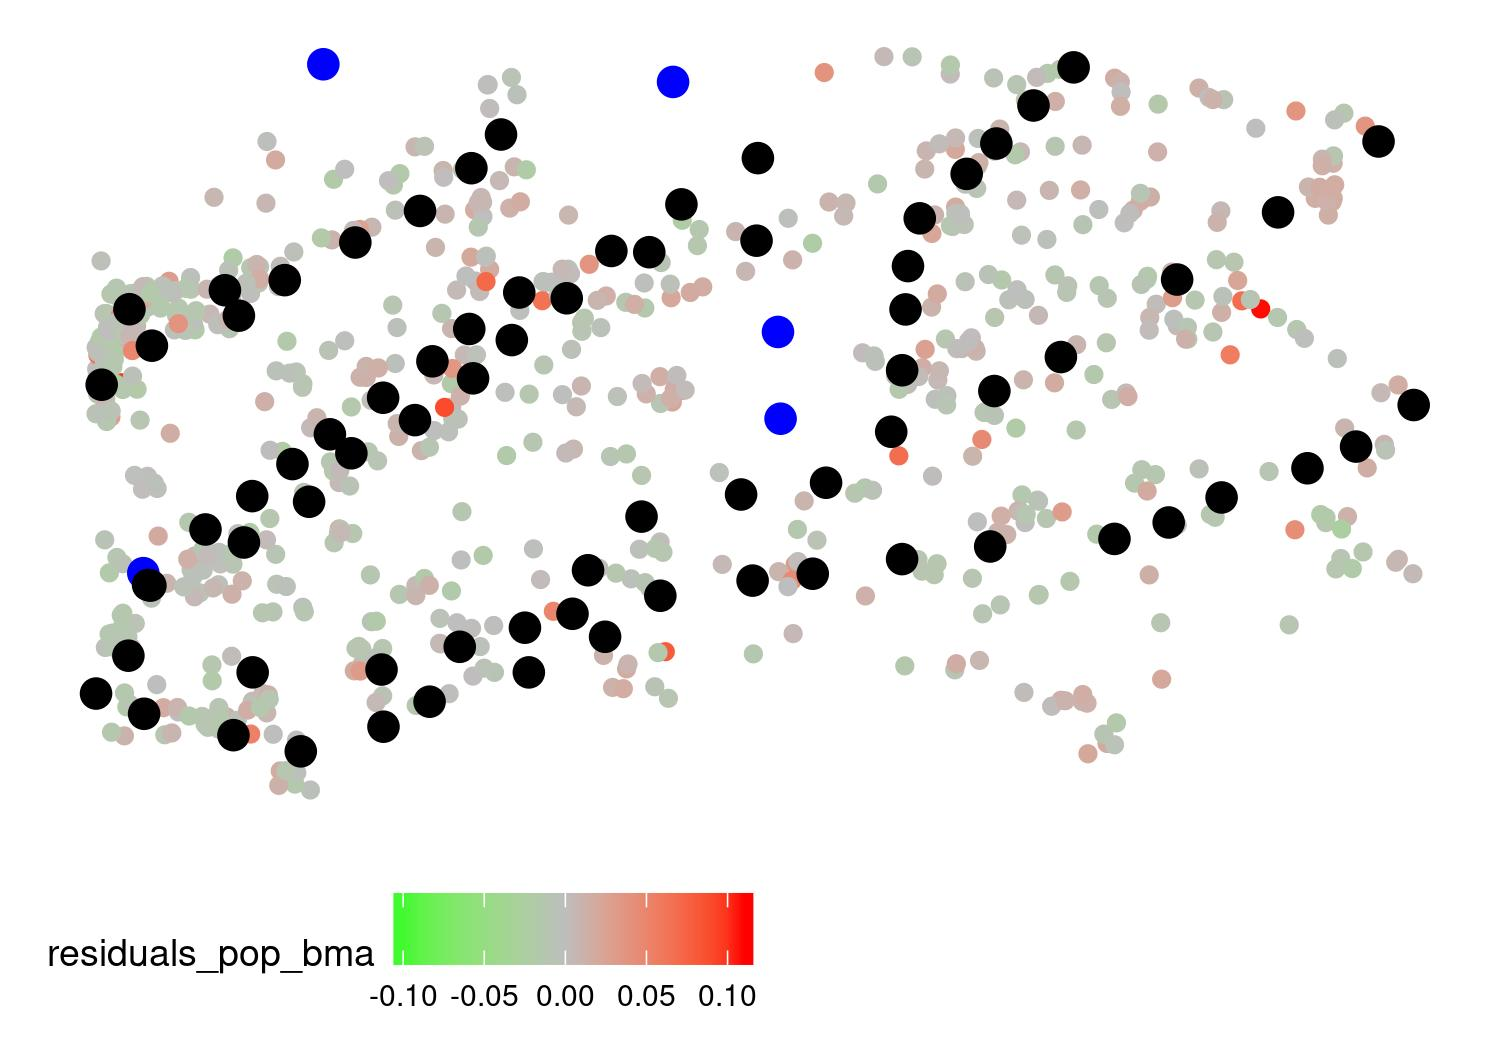
\includegraphics[scale = 0.8]{map_pop_bma.jpeg}
\end{frame} 




\end{document}
